\documentclass[]{beamer}
\mode<presentation>
{
% use attribute "dark" for dark theme
% use attribute "contrast" for maximum text contrast
\usetheme[]{wlansi}
\usefonttheme[onlymath]{serif}
\setbeamercovered{transparent}
}  

\usepackage{hyperref}
\usepackage[utf8]{inputenc}
\usepackage{mathptmx}
\usepackage{xmpmulti}
\usepackage[T1]{fontenc}
\usepackage[utf8]{inputenc}
\usepackage{cmap}
\usepackage{ifthen}
\usepackage{type1ec}
\usepackage{concrete}
\usepackage{tikz}
\usetikzlibrary{positioning,arrows,decorations.pathreplacing,decorations.text,shapes,calc,fit}

\DeclareFontFamily{T1}{ccr}{}
\DeclareFontShape{T1}{ccr}{m}{n}{<5><6><7><8><9><10>gen*eorm<10->eorm10}{}
\DeclareFontShape{T1}{ccr}{m}{sl}{<5><6><7><8><9><10>gen*eosl<10->eosl10}{}
\DeclareFontShape{T1}{ccr}{m}{it}{<->eoti10}{}
\DeclareFontShape{T1}{ccr}{m}{sc}{<->eocc10}{}
\DeclareFontShape{T1}{ccr}{bx}{n}{<->ssub*cmr/bx/n}{}
\DeclareFontShape{T1}{ccr}{bx}{sl}{<->ssub*cmr/bx/sl}{}
\DeclareFontShape{T1}{ccr}{bx}{it}{<->ssub*cmr/bx/it}{}
\DeclareFontShape{T1}{ccr}{sbc}{n}{<->ssubf*ecssdc10}{}
\usepackage[T1]{fontenc}
\renewcommand{\sfdefault}{\rmdefault}
\renewcommand{\familydefault}{\rmdefault}
\renewcommand{\bfdefault}{m}
\newcommand{\nodewatcher}{\emph{nodewatcher }}
\newcommand{\wlanslovenija}{\emph{wlan slovenija }}

\newcommand{\ifstrempty}[3]{%
\def\reallyempty{}%
\def\ifarg{#1}%
\ifx\ifarg\reallyempty%
{#2}
\else
{#3}
\fi%
}

\newcommand{\wrapframe}[1]{
\begin{frame}
 #1
\end{frame}
}

\newenvironment{changemargin}[2]{%
\begin{list}{}{%
\setlength{\topsep}{0pt}%
\setlength{\leftmargin}{#1}%
\setlength{\rightmargin}{#2}%
\setlength{\listparindent}{\parindent}%
\setlength{\itemindent}{\parindent}%
\setlength{\parsep}{\parskip}%
}%
\item[]}{\end{list}}

\newcommand{\simpleslide}[3]{\wrapframe{
\ifstrempty{#1}{\vbox{ \ } 

}{
{\footnotesize #1}
} \vfill

\begin{center}
#2
\end{center}
\vfill
\ifstrempty{#3}{ \ }{
\begin{flushright}
{\footnotesize #3}
\end{flushright}
}
}}

\newcommand{\simpleslideimage}[2]{\wrapframe{
\begin{center}
\includegraphics[width=0.8\paperwidth,height=0.6\paperheight,keepaspectratio]{#1}
\\ {\footnotesize #2}
\end{center}}
}

\newcommand{\fullslideimage}[1]{
\begin{frame}[plain]
\begin{changemargin}{-1cm}{-1cm}
\begin{center}
\includegraphics[width=\paperwidth,height=\paperheight,keepaspectratio]{#1}
\end{center}
\end{changemargin}
\end{frame}
}

\newcommand{\rightfooter}[1]{\vfill\hfill #1}

\title{Omrežje \wlanslovenija}

\subtitle{Jernej Kos \\ Piškot FRI}

%\author{}

%\institute{}

\date[]{5.3.2015}

\tikzstyle{vertex}=[circle,text=blue!75,fill=blue!25,minimum size=20pt,inner sep=0pt]
\tikzstyle{selected vertex} = [vertex, fill=red!24, text=red]
\tikzstyle{edge} = [draw=black,thick,-]
\tikzstyle{weight} = [font=\scriptsize]
\tikzstyle{selected edge} = [draw,line width=5pt,-,red!50]
\tikzstyle{destination} = [vertex,fill=orange!24, text=orange]

\begin{document}

% makes a title slide
\maketitle

\pgfdeclarelayer{background}
\pgfsetlayers{background,main}

\simpleslide{}{\wlanslovenija -- odprto brezžično omrežje Slovenije \\ https://wlan-si.net}{https://grow.wlan-si.net \\ https://dev.wlan-si.net}

\simpleslide{}{Pobuda za izgradnjo odprtega brezžičnega \\
omrežja po Sloveniji, temelječega na sodelovanju, \\
izmenjavi znanja in izkušenj ter skupnosti.}{}

%TODO primerjava s tradicionalnim pristopom
\simpleslide{Organska rast omrežne infrastrukture.}{Izzivi.}{Koordinacija skupnosti.}

\simpleslide{Omrežje.}{Mesh omrežje.}{Brezžično mesh omrežje.}

\simpleslide{Mesh omrežje.}{

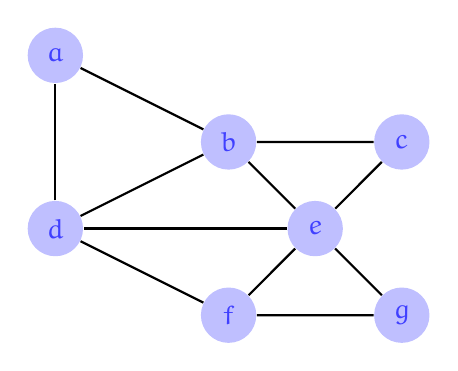
\begin{tikzpicture}[scale=1.1,auto,swap]
  \foreach \pos / \name in {{(0,2)/a}, {(2,1)/b}, {(4,1)/c},
                            {(0,0)/d}, {(3,0)/e}, {(2,-1)/f}}
    \node[vertex] (\name) at \pos {$\name$};
  
  \node[vertex] (g) at (4,-1) {$g$};
  
  % Connect vertices with edges
  \foreach \source / \dest in {b/a, c/b, d/a, d/b,
                               e/b, e/c, e/d,
                               f/d, f/e, g/e, g/f}
      \path[edge] (\source) -- (\dest);
\end{tikzpicture}

}{Peer-to-peer.}

\fullslideimage{images/network_topology.png}

\simpleslide{Omrežje.}{Povezljivost na katerikoli možen način.}{WiFi, Ethernet, L2TPv3, KORUZA...}

\fullslideimage{images/node-map-slovenia.png}

\fullslideimage{images/node-map-haloze.png}

\simpleslide{Omrežje.}{Dinamično usmerjanje, protokoli.}{OLSR, Babel, BATMAN, BMX6, 802.11s.}

\simpleslide{Najkvalitetnejša pot med točkama $a$ in $g$.}{

\begin{tikzpicture}[scale=1.8,auto,swap]
  \foreach \pos / \name in {{(0,2)/a}, {(2,1)/b}, {(4,1)/c},
                            {(0,0)/d}, {(3,0)/e}, {(2,-1)/f}}
    \node[vertex] (\name) at \pos {$\name$};
  
  \node[destination] (g) at (4,-1) {$g$};
  
  % Connect vertices with edges and draw weights
  \foreach \source / \dest / \weight in {b/a/$1.0$, c/b/$1.0$, d/a/$1.21$, d/b/$2.33$,
                                         e/b/$2.17$, e/c/$2.43$, e/d/$1.87$,
                                         f/d/$7.81$, f/e/$3.20$,
                                         g/e/$2.01$, g/f/$1.12$}
      \path[edge] (\source) -- node[weight] {$\weight$} (\dest);
  
  \foreach \vertex in {a,d,e}
    \path<2-> node[selected vertex] at (\vertex) {$\vertex$};
  
  \begin{pgfonlayer}{background}
    \foreach \source / \dest in {a/d,d/e,e/g}
      \path<2->[selected edge] (\source.center) -- (\dest.center);
  \end{pgfonlayer}
\end{tikzpicture}

}{}

\simpleslide{Brezžično omrežje.}{Metrike.}{ETX, ETT, RTT.}

\simpleslideimage{images/battlemeshv8_logo.png}{Protokoli, metrike. Kateri je ``boljši''? \\ http://battlemesh.org/}

\simpleslide{Omrežje.}{Naprave.}{Linux, OpenWrt. \\ http://www.openwrt.org}

\simpleslideimage{images/wr741nd-4v20-4.jpg}{}

\simpleslideimage{images/aggregator.jpg}{}

\simpleslide{$\sim$ 1000 geografsko razpršenih točk.}{Naprave. Konfiguracija. Postavitev.}{Upravljanje omrežja.}

\simpleslide{Upravljanje omrežja.}{\huge \nodewatcher}{Razširljiva platforma za upravljanje \\ velikih (brezžičnih) mesh omrežij.}

\simpleslideimage{clipart/device-mgmt-cycle.pdf}{Cikel upravljanja naprav.}

\simpleslide{}{Konfiguracija.}{Neodvisna od platforme.}

\simpleslide{Firmware.}{Transformacija konfiguracije.}{Generator.}

\fullslideimage{images/firmware-buildsystem.pdf}

\simpleslide{}{Postavitev.}{}

\fullslideimage{images/neubergerjeva.jpg}

\fullslideimage{images/glinska.jpg}

\fullslideimage{images/rozmanova-1.jpg}

\fullslideimage{images/rozmanova-2.jpg}

\fullslideimage{images/urban.jpg}

\fullslideimage{images/urban2.jpg}

\fullslideimage{images/linkslatinaurban06.jpg}

\fullslideimage{images/PohorjeTestiranje.png}

\fullslideimage{images/solar-1.jpg}

\fullslideimage{images/solar-2.jpg}

\fullslideimage{images/koruza-ijs-teslova-4.jpg}

\simpleslide{Nadzor.}{Podatki.}{Skladnost s konfiguracijo. \\ Samodejno odkrivanje napak v omrežju.}

\simpleslide{Pridobivanje podatkov.}{nodewatcher-agent, \\ SNMP, \\ ...}{Modularna platforma.}

\fullslideimage{images/monitoring-pipeline.pdf}

\fullslideimage{images/datastream-storage.pdf}

\fullslideimage{images/datastream-counter-reset.pdf}

\fullslideimage{images/implementation-interactive-visualization.png}

\simpleslide{Vse le ne gre brez žic.}{{\huge \textit{Tunneldigger}} \\ {...in zakaj ne OpenVPN?}}{L2TPv3 broker in odjemalec.}

%TODO slika s shemo vpn?

\simpleslide{Tunneldigger. Layer 2 pseudo-wire.}{Context switchi, kopiranje. \\ L2TPv3 podpora v Linux jedru.}{NAT, PMTU, ...}

\subtitle{https://wlan-si.net \\ jernej@kos.mx}
\date[]{}

\maketitle

\end{document}
